\chapter{Clustering and Classification}

Even though supervised learning is the most common type of machine learning, unsupervised learning is the most common type of learning in the world. Therefore, not only supervised but also unsupervised learning is important to understand. The two main techniques used for unsupervised and supervised learning are, respectively, clustering and classification. In this chapter, we will discuss these two techniques in detail.

\section{Clustering}

Clustering is a technique used to group similar data points together. During the following sections, we will discuss some of the most common clustering algorithms, including K-Means, Hierarchical Clustering, and DBSCAN.

\subsection{K-Means}

K-Means is a popular clustering algorithm that partitions the data into $k$ clusters. The exact division of the data into clusters is determined by different algorithms that soon will be discussed; however, it has the following general disadvantages:
\begin{itemize}
    \item The number of clusters $k$ must be specified beforehand, which can be difficult to determine. In order to determine the optimal number of clusters, techniques such as the Elbow Method can be used.
    
    The Elbow Method involves plotting the WCSS (Within-Cluster Sum of Squares) against the number of clusters $k$. The WCSS measures the total distance between each point and the centroid of its assigned cluster. This plot is always decreasing as $k$ increases, but the goal is to find the point where the rate of decrease sharply changes, resembling an ``elbow''. This point indicates the optimal number of clusters, as adding more clusters beyond this point does not significantly reduce the WCSS.
    \item K-Means only works well with spherical clusters (if the euclidean distance is used) or cubical clusters (if the Manhattan distance is used). It may not perform well with clusters of arbitrary shapes.
    \item K-Means is sensitive to the initial placement of centroids, which can lead to different results on different runs. If the initial centroids are chosen within the same cluster, the algorithm may converge to a local minimum. Different initialization methods, such as K-Means++, can be used to improve the convergence and stability of the algorithm.
\end{itemize}

It has several specific applications, such as image compression:
\begin{itemize}
    \item In image compression, K-Means can be used to reduce the number of colors in an image. Each pixel's color is treated as a data point in a three-dimensional space (representing the RGB color values). K-Means clusters these colors into $k$ groups, and each pixel is then assigned the color of its corresponding cluster centroid. This results in a compressed image with fewer colors while maintaining visual similarity to the original.
\end{itemize}

Some of the algorithms used to determine the clusters in K-Means include:
\subsubsection{Lloyd's Algorithm}
Lloyd's Algorithm is the most common algorithm used for K-Means clustering. It works as follows:
\begin{enumerate}
    \item Initialize $k$ centroids randomly. They can be selected randomly from the data points or generated randomly within the data space.
    \item Assign each data point to the nearest centroid, forming $k$ clusters.
    \begin{equation*}
        C_i = \{x_j : \|x_j - \mu_i\|^2 \leq \|x_j - \mu_k\|^2, \forall k, 1 \leq k \leq K\}
    \end{equation*}
    where $C_i$ is the set of data points assigned to cluster $i$, $x_j$ is a data point, $\mu_i$ is the centroid of cluster $i$, and $\|\cdot\|$ denotes a distance (usually Euclidean).
    \item Update the centroids by calculating the mean of the data points in each cluster:
    \begin{equation*}
        \mu_i = \frac{1}{|C_i|} \sum_{x_j \in C_i} x_j
    \end{equation*}
    \item Repeat steps 2 and 3 until convergence, which occurs when the centroids do not change significantly or a maximum number of iterations is reached.
\end{enumerate}

This algorithm is efficient and works well for many datasets, but it can converge to a local minimum, which is why the initialization of centroids is crucial.

\subsubsection{MacQueen's Algorithm}
MacQueen's Algorithm is a different approach to K-Means clustering that updates the centroids incrementally as data points are assigned to clusters. It works as follows:
\begin{enumerate}
    \item Select the first $k$ data points as the initial centroids.
    \item For each data point, assign it to the nearest centroid and update the centroid's position immediately after the assignment. The update is done using the following formula:
    \begin{equation*}
        \mu_{\text{new}} = \mu_{\text{old}} + \frac{x_j - \mu_{\text{old}}}{n_i + 1}
    \end{equation*}
    where $\mu_{\text{old}}$ is the current centroid, $x_j$ is the new data point being assigned, and $n_i$ is the number of data points currently assigned to that centroid before the new assignment. This formula updates the centroid by moving it towards the new data point, taking into account the number of points already assigned to that cluster.
    \item Repeat this process for all data points until convergence, which occurs when the centroids do not change significantly or a maximum number of iterations is reached.
\end{enumerate}

This algorithm can be more efficient than Lloyd's Algorithm for large datasets, as it updates the centroids incrementally rather than waiting for all data points to be assigned before updating.

\subsubsection{Jenks-Caspall Algorithm}

The Jenks-Caspall Algorithm is a method used for optimizing the classification of data into clusters, particularly in the context of choropleth maps. Its aim is to use the \emph{natural breaks} in the data to determine the optimal number of clusters and their boundaries, achieving two main objectives:
\begin{itemize}
    \item Minimize the variance within each cluster, ensuring that data points within the same cluster are as similar as possible.
    \item Maximize the variance between clusters, ensuring that different clusters are as distinct as possible.
\end{itemize}

It works in two main cycles:
\begin{enumerate}
    \item \ul{Re-iterative Cycling}: Use the previously explained algorithms (Lloyd's or MacQueen's) to determine the clusters and their centroids. This process may be repeated multiple times to refine the clusters and improve the classification.
    \item \ul{Forced Cycling}: This step involves forcing the algorithm to consider different cluster boundaries by adjusting the centroids and reassigning data points. This can help to escape local minima and find a more optimal clustering solution.
\end{enumerate}

\subsubsection{Otsu's method}

Otsu's method is a technique used for image thresholding, which can be considered a form of clustering in the context of image processing. It works by finding the optimal threshold that separates the pixel intensity values into two classes (foreground and background) while maximizing the between-class variance.

\subsubsection{X-Means}
X-Means is an extension of the K-Means algorithm that automatically determines the optimal number of clusters. It works by starting with a small number of clusters ($k=2$) and then iteratively splitting clusters based on a criterion such as the Bayesian Information Criterion (BIC)\footnote{The WCSS can't be used, as it always decreases.}. The BIC is a statistical measure that:
\begin{itemize}
    \item Penalizes the complexity of the model (number of clusters) to avoid overfitting.
    \item Rewards the goodness of fit of the model to the data.
\end{itemize}

For each cluster, two options are evaluated:
\begin{itemize}
    \item Keep the cluster as it is.
    \item Split the cluster into two sub-clusters and evaluate the BIC for both the original and the split clusters.
\end{itemize}
If the BIC improves after splitting, the cluster is split; otherwise, it remains unchanged.

\subsubsection{K-Means++}
K-Means++ is an initialization method for the K-Means algorithm that aims to improve the convergence and stability of the algorithm by selecting initial centroids in a more strategic way. The process works as follows:
\begin{enumerate}
    \item Randomly select the first centroid from the data points.
    \item For each subsequent centroid, select a data point with a probability proportional to the square of the distance ($d^2$) from the nearest existing centroid. This means that data points that are farther away from the existing centroids are more likely to be selected as new centroids.
    \item Repeat this process until $k$ centroids have been selected.
\end{enumerate}

This solves an important problem of the K-Means algorithm, which is the sensitivity to the initial placement of centroids. If two centroids are initialized within the same cluster, the algorithm may converge to a local minimum. By using K-Means++, the initial centroids are more likely to be spread out across the data space, leading to better convergence and improved clustering results.

\subsubsection{K-Medians}

K-Medians is a variant of the K-Means algorithm that uses the median instead of the mean to update the centroids. This makes it more robust to outliers, as the median is less affected by extreme values than the mean.

\subsubsection{K-Medoids}

K-Medoids (also known as PAM - Partitioning Around Medoids) is another variant of the K-Means algorithm that uses actual data points (medoids) as the centroids instead of calculating the mean or median. This can be more robust to outliers and can work better with non-spherical clusters. The algorithm works as follows:
\begin{enumerate}
    \item Initialize $k$ medoids randomly from the data points.
    \item Assign each data point to the nearest medoid, forming $k$ clusters.
    \item In each cluster, select the data point that minimizes the total distance to all other points in the cluster as the new medoid.
\end{enumerate}
This process is repeated until the medoids do not change, indicating convergence.

% // TODO: Minimizar varianza? Distancia? Qué en cada caso?

\subsection{Hierarchical Clustering}

Hierarchical Clustering is a method of cluster analysis that builds a hierarchy of clusters. It can be divided into two main types:
\begin{itemize}
    \item \ul{Agglomerative Clustering}: This is a bottom-up approach where each data point starts as its own cluster, and pairs of clusters are merged as one moves up the hierarchy. The merging process continues until all data points are in a single cluster or until a specified number of clusters is reached.
    \item \ul{Divisive Clustering}: This is a top-down approach where all data points start in a single cluster, and the cluster is recursively split into smaller clusters until each data point is in its own cluster or until a specified number of clusters is reached.
\end{itemize}

The structure of the hierarchy can be represented as a \emph{dendrogram}, which is a tree-like diagram that shows the arrangement of the clusters formed at each step of the algorithm. The height of the branches in the dendrogram represents the distance or dissimilarity between clusters, allowing for the visualization of how clusters are merged or split. This method is sensitive to outliers, as they can significantly affect the structure of the hierarchy and the resulting clusters.

Since divisive clustering is only seldomly used, in the following sections different linkage criteria for agglomerative clustering will be discussed. In each step of the agglomerative clustering process, the two clusters that are closest to each other are merged (so the number of clusters decreases by one). The distance between clusters can be defined in different ways, leading to different linkage criteria.

\subsubsection{Single Linkage}
In single linkage, the distance between two clusters is defined as the minimum distance between any two points in the two clusters.
\begin{equation*}
    d_{\text{single}}(A, B) = \min_{a\in A, b\in B} d(a, b)
\end{equation*}

This method can lead to the \emph{chaining effect}, where clusters can be formed by a series of close points, even if the overall clusters are not well separated. The reason for this is that single linkage focuses on the closest points between clusters, which can result in elongated and irregularly shaped clusters.

\subsubsection{Complete Linkage}

In complete linkage, the distance between two clusters is defined as the maximum distance between any two points in the two clusters.
\begin{equation*}
    d_{\text{complete}}(A, B) = \max_{a\in A, b\in B} d(a, b)
\end{equation*}

This method tends to produce more compact and spherical clusters, as it considers the farthest points between clusters. However, it can be sensitive to outliers, as a single outlier can significantly increase the distance between clusters.

\subsubsection{Average Linkage}

In average linkage, the distance between two clusters is not decided by just two points, but rather by all the points in the clusters. There are different specific ways to define the average distance:
\begin{itemize}
    \item \ul{Unweighted Average Linkage}: The distance between two clusters is defined as the average distance between all pairs of points in the two clusters.
    \begin{equation*}
        d_{\text{unweighted}}(A, B) = \frac{1}{|A|\cdot |B|} \sum_{a\in A,\ b\in B} d(a, b)
    \end{equation*}
    
    \item \ul{Weighted Average Linkage}: The distance between two clusters is defined as the average distance between all pairs of points in the two clusters, but with weights assigned to the distances based on the size of the clusters.
    \begin{equation*}
        d_{\text{weighted}}(A, B) = \frac{|A|}{|A| + |B|} d_{\text{unweighted}}(A, B) + \frac{|B|}{|A| + |B|} d_{\text{unweighted}}(B, A)
    \end{equation*}

    % // TODO: Diferencia con el anterior? Xq?
    % $\frac{d(A,C) + d(B,C)}{2}$ Y esto?

    \item \ul{Centroid Method Unweighted Pair-Group Method using Centroids}:
    The distance between two clusters is defined as the distance between their centroids. The centroid of a cluster is the mean of all the points in the cluster.
    \begin{equation*}
        d_{\text{centroid}}(A, B) = d(\mu_A, \mu_B)
    \end{equation*}
    where $\mu_A$ and $\mu_B$ are the centroids of clusters $A$ and $B$, respectively.

    \item \ul{Median Method Weighted Pair-Group Method using Medians}:
    The distance between two clusters is defined as the distance between their medians. The median of a cluster is the median of all the points in the cluster.
    \begin{equation*}
        d_{\text{median}}(A, B) = d(\text{median}(A), \text{median}(B))
    \end{equation*}

    \item \ul{Ward's Method}: This method minimizes the total within-cluster variance. The distance between two clusters is defined as the increase in the total within-cluster variance that would result from merging the two clusters.
    \begin{equation*}
        d_{\text{ward}}(A, B) = \frac{|A| \cdot |B|}{|A| + |B|} d_{\mu_A, \mu_B}^2
    \end{equation*}

    This method tends to produce clusters of similar size and can be more effective in identifying compact clusters. The reason for this is that Ward's method focuses on minimizing the variance within clusters, which encourages the formation of clusters that are more homogeneous and compact.
\end{itemize}

This method provides a compromise between single and complete linkage, as it considers the overall distance between clusters rather than just the closest or farthest points. It can produce clusters that are more balanced in terms of shape and size.

\subsection{DBSCAN}

DBSCAN (Density-Based Spatial Clustering of Applications with Noise) is a density-based clustering algorithm that groups together data points that are closely packed together, while marking points that lie alone in low-density regions as outliers. It works based on two parameters:
\begin{itemize}
    \item \ul{Epsilon ($\varepsilon$)}: This parameter defines the radius of the neighborhood around a data point. It determines how close points need to be to each other to be considered part of the same cluster.
    \item \ul{\texttt{MinPts}}: This parameter defines the minimum number of points required to form a dense region.
\end{itemize}

The algorithm classifies data points into three categories:
\begin{itemize}
    \item \ul{Core Points}: These are points that have at least \texttt{MinPts} points within their $\varepsilon$-neighborhood. Core points are the central points of clusters.
    \item \ul{Border Points}: These are points that have fewer than \texttt{MinPts} points within their $\varepsilon$-neighborhood but are within the $\varepsilon$-neighborhood of a core point. Border points are on the edge of clusters.
    \item \ul{Noise Points}: These are points that do not have enough neighboring points to be classified as core points and are not within the $\varepsilon$-neighborhood of any core point. Noise points are considered outliers.
\end{itemize}

The DBSCAN algorithm works as follows:
\begin{enumerate}
    \item For each unvisited point, check if it is a core point by counting the number of points within its $\varepsilon$-neighborhood.
    \begin{itemize}
        \item If the point is a core point, create a new cluster. All points that are density-reachable from this core point (i.e., all points that can be reached by traversing through core points) are added to the cluster.
        \item If the point is a border point, it is not computed. It will be considered when its associated core point is processed.
        \item If the point is a noise point, it is marked as an outlier and is not included in any cluster.
    \end{itemize}
    \item Repeat this process until all points have been visited.
\end{enumerate}

It has some advantages over other clustering algorithms, as it can find clusters of arbitrary shapes and is robust to outliers. However, it can be sensitive to the choice of parameters ($\varepsilon$ and \texttt{MinPts}), and it may not perform well with varying densities of clusters.

\subsection{OPTICS}

OPTICS (Ordering Points To Identify the Clustering Structure) is an extension of the DBSCAN algorithm that addresses some of its limitations, particularly in handling clusters of varying densities. It uses two parameters similar to DBSCAN:
\begin{itemize}
    \item \ul{Epsilon ($\varepsilon$)}: This parameter defines the maximum radius of the neighborhood around a data point. It is used to avoid a core point to search for neighbors indefinitely, which can lead to performance issues.
    \item \ul{\texttt{MinPts}}: This parameter defines the minimum number of points required to form a dense region, also similar to DBSCAN.
\end{itemize}

The OPTICS algorithm introduces two new concepts to better capture the clustering structure:

\begin{itemize}
    \item \ul{Core Distance}: This is the distance from a point to its \texttt{MinPts}-th nearest neighbor. If a point has fewer than \texttt{MinPts} neighbors within $\varepsilon$, its core distance is undefined (or set to $\infty$).
    \begin{equation*}
        d_{\text{core}}(p) = \begin{cases}
            \text{distance to the } \texttt{MinPts}-\text{th nearest neighbor of } p & \text{if } |N_{\varepsilon}(p)| \geq \texttt{MinPts} \\
            \infty & \text{otherwise}
        \end{cases}
    \end{equation*}
    \item \ul{Reachability Distance}: This is the distance from a point $p$ to another point $o$ that is reachable from $p$. It is defined as:
    \begin{equation*}
        d_{\text{reachability}}(p, o) = \max(d_{\text{core}}(p), d(p, o))
    \end{equation*}

    The maximum function ensures that the reachability distance reflects both the core distance of $p$ and the actual distance between $p$ and $o$. If both points are close in a dense region, the reachability distance is set to the core distance, which helps to identify clusters of varying densities (as every core point in the same cluster will have similar core distances). If the points are farther apart, the reachability distance will reflect the actual distance between them, which helps to distinguish between different clusters.
\end{itemize}

The OPTICS algorithm uses two different lists to keep track of the points:
\begin{itemize}
    \item An ordered list of points, which maintains the order in which points are processed. It contains all the points in the dataset and their corresponding reachability distances when they are added to the list. The order of points in this list does not change once they are added.
    \item A priority queue of points to be processed, which is ordered by their reachability distance. Points with lower reachability distances have higher priority and are processed first.
\end{itemize}

Using those two lists, the OPTICS algorithm works as follows:
\begin{enumerate}
    \item A not processed point is selected and added to the ordered list with a reachability distance of $\infty$ (as a second point would be needed to calculate the reachability distance). If it is a core point, all its \texttt{MinPts} neighbors are added to the priority queue with their reachability distances from the selected core point.
    \begin{itemize}
        \item The first point in the priority queue is selected and added to the ordered list. If it is a core point, all its \texttt{MinPts} neighbors are added to the priority queue with their reachability distances from the selected core point (if they were already in the priority queue, their reachability distance is updated if the new reachability distance is smaller).
    \end{itemize}
    \item That process is repeated until the priority queue is empty, and then the first step is repeated again. This process continues until all points have been processed and added to the ordered list.
\end{enumerate}

After processing all points, a reachability plot can be created, which is a visual representation of the reachability distances of the points in the order they were processed.
\begin{itemize}
    \item \ul{X-axis}: The points ordered by the order in which they were processed (i.e., the order in which they were added to the ordered list).
    \item \ul{Y-axis}: The reachability distance of each point.
\end{itemize}

In the reachability plot, clusters can be identified as valleys (regions of low reachability distance) separated by peaks (regions of high reachability distance). A really dense cluster will have a long valley with low reachability distances, while a less dense cluster will have a shorter valley with higher reachability distances. Noise points will appear as peaks in the reachability plot, as they have high reachability distances. An example of a reachability plot is shown in the Figure~\ref{fig:reachability_plot}.
\begin{figure}
    \centering
    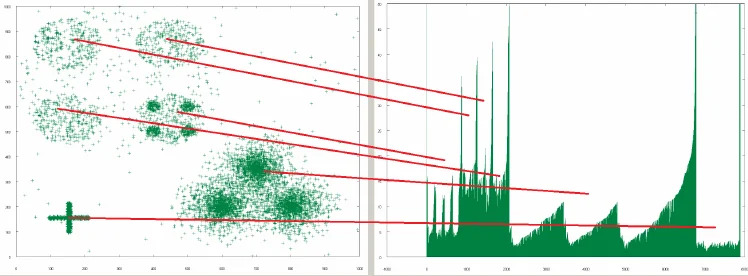
\includegraphics[width=0\textwidth]{./images/OPTICS.jpg}
    \caption{Example of a reachability plot. The valleys represent clusters, while the peaks represent noise points.}
    \label{fig:reachability_plot}
\end{figure}

This method allows for the identification of clusters of varying densities, as the reachability distances will reflect the density of the clusters. It has however a big disadvantage, which is that it has a subjective component in the interpretation of the reachability plot, as it can be difficult to determine where the valleys and peaks are, especially in cases where the clusters are not well defined.

\section{Classification}

\subsection{K-Nearest Neighbors}